\documentclass[notes,aspectratio=169]{beamer}
\usepackage[utf8]{inputenc}
\usepackage[T1]{fontenc}
\usepackage{circuitikz}

\title{IL2234 - Digital Design with HDL}
\subtitle{Lecture 1 - Introduction}
% \date[ISPN ’80]{27th International Symposium of Prime Numbers}
% \author[Euclid]{Euclid of Alexandria \texttt{euclid@alexandria.edu}}
\author[J. Altayó]{Jordi Altayó - \texttt{jordiag@kth.se}}

\usetheme{kth}

\newcommand{\subb}[1]{_{\text{#1}}}
\setbeamertemplate{note page}[plain]
\begin{document}

\begin{frame}[plain]
\titlepage
\end{frame}

\begin{frame}
\frametitle{There Is No Largest Prime Number}
\framesubtitle{The proof uses \textit{reductio ad absurdum}.}
\begin{theorem}
There is no largest prime number.
\end{theorem}
\begin{proof}
\begin{enumerate}
\item<1-| alert@1> Suppose $p$ were the largest prime number.
\item<2-> Let $q$ be the product of the first $p$ numbers.
\item<3-> Then $q+1$ is not divisible by any of them.
\item<1-> But $q+1$ is greater than $1$, thus divisible by some prime number not in the first $p$ numbers.
  \end{enumerate}
\end{proof}
\end{frame}

\begin{frame}
  \frametitle{There tete}
  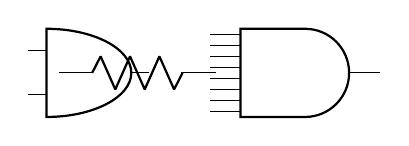
\begin{tikzpicture}
    \draw (0,0) to[R] (2,0);
    \node [american and port] at (1,0) {};
    \node [ieeestd and port, number inputs=8] at (3,0) {};
  \end{tikzpicture}
\end{frame}

\begin{frame}
  \frametitle{CMOS equivalent circuit}
  \centering
  \resizebox{!}{6cm}{%
    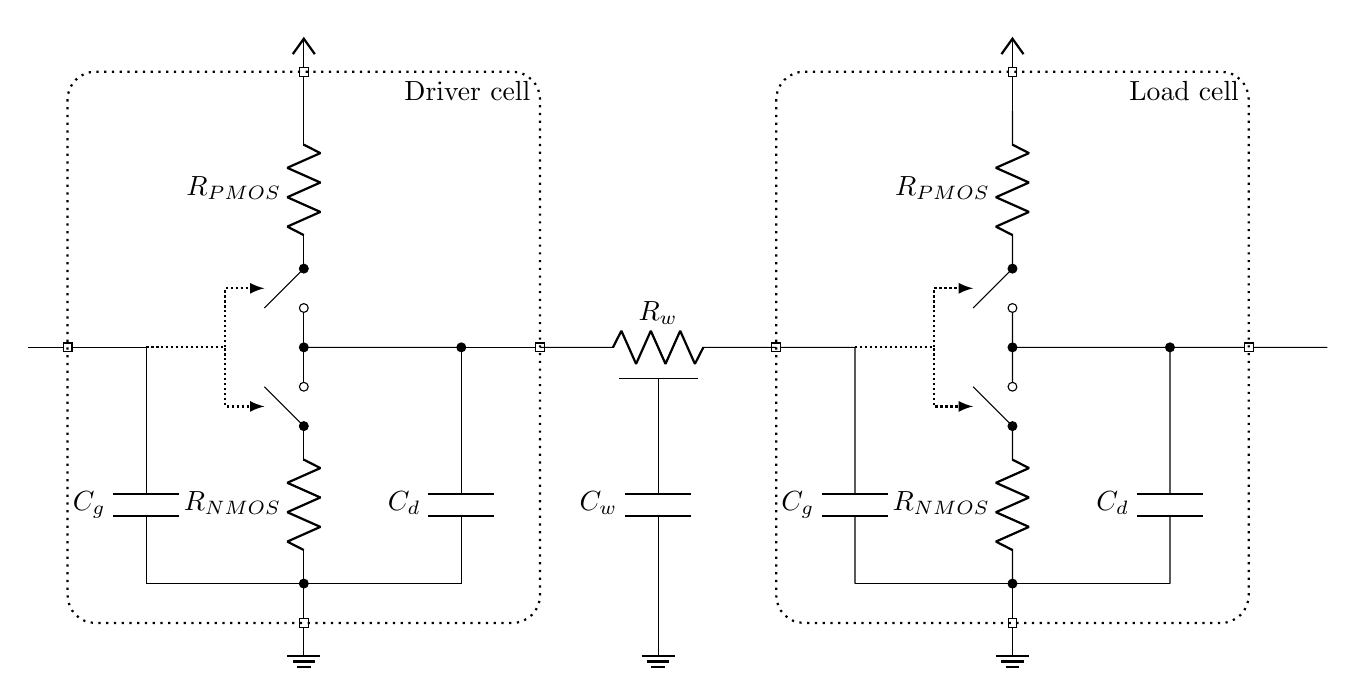
\begin{tikzpicture}
      \draw (4,-1) -- (5,-1) -- (5, -2) to[C, l_=$C\subb{g}$] (5,-4);
      \draw (7,-4) to[R, -*, l=$R\subb{NMOS}$] (7,-2);
      \draw (9,-4) to[C, l=$C\subb{d}$] (9,-2) -- (9,-1) -- (11,-1);
      \draw (5,-4) to[short, -*,] (7,-4) -- (9,-4);
      \draw (7,-4) -- (7,-4.5) node[ground] {};
      \draw (7,-1) to[short, *-*] (9,-1);
      \draw (7,-1.5) to[short, o-o] (7,-0.5);
      \draw (7,-2) -- (6.5,-1.5) (6.5,-0.5) -- (7,0);
      \draw [thick, densely dotted, -latex] (5,-1) -- (6,-1) -- (6,-1.75) -- (6.5,-1.75);
      \draw [thick, densely dotted, -latex] (6,-1) -- (6,-0.25) -- (6.5,-0.25);
      \draw (7,0) to[R, *-, l=$R\subb{PMOS}$] (7,2);
      \draw (7,2) -- (7,2.5) node[vcc] {};
      \node [osquarepole] at (4,-1) {};
      \node [osquarepole] at (7,-4.5) {};
      \node [osquarepole] at (10,-1) {};
      \node [osquarepole] at (7,2.5) {};
      \draw [thick, dotted, rounded corners=10pt] (4,2.5) rectangle (10,-4.5);
      \node[anchor=north east] at (10,2.5) {Load cell};

      \draw (-5.5,-1) -- (-4,-1) -- (-4, -2) to[C, l_=$C\subb{g}$] (-4,-4);
      \draw (-2,-4) to[R, -*, l=$R\subb{NMOS}$] (-2,-2);
      \draw (0,-4) to[C, l=$C\subb{d}$] (0,-2) -- (0,-1) -- (1,-1);
      \draw (-4,-4) to[short, -*,] (-2,-4) -- (0,-4);
      \draw (-2,-4) -- (-2,-4.5) node[ground] {};
      \draw (-2,-1) to[short, *-*] (0,-1);
      \draw (-2,-1.5) to[short, o-o] (-2,-0.5);
      \draw (-2,-2) -- (-2.5,-1.5) (-2.5,-0.5) -- (-2,0);
      \draw [thick, densely dotted, -latex] (-4,-1) -- (-3,-1) -- (-3,-1.75) -- (-2.5,-1.75);
      \draw [thick, densely dotted, -latex] (-3,-1) -- (-3,-0.25) -- (-2.5,-0.25);
      \draw (-2,0) to[R, *-, l=$R\subb{PMOS}$] (-2,2);
      \draw (-2,2) -- (-2,2.5) node[vcc] {};
      \node [osquarepole] at (-5,-1) {};
      \node [osquarepole] at (-2,-4.5) {};
      \node [osquarepole] at (1,-1) {};
      \node [osquarepole] at (-2,2.5) {};
      \draw [thick, dotted, rounded corners=10pt] (-5,2.5) rectangle (1,-4.5);
      \node[anchor=north east] at (1,2.5) {Driver cell};


      \draw (4,-1) to[R, l_=$R\subb{w}$, name=Rint] (1,-1);
      \draw (Rint) ++ (0,-0.4) ++(0.5,0) --++(-1,0) ++(0.5,0) --++ (0,-0.6) to[C, l_=$C\subb{w}$] ++ (0,-2) -- ++(0,-0.5) node[ground] {};
    \end{tikzpicture}
  }

  
\end{frame}

\end{document}
